\chapter{Mapping between Morita equivalent string-net states with a constant depth quantum circuit}\label{app:SN}
\section{Synopsis}
As argued in \cref{eq:SymGappedPhases}, two models belong to the same gapped quantum phase of matter if they are related by an interpolating quantum circuit of sublinear depth. In this project, we explicitly construct such a constant-depth circuit for string-net models whose input UFCs $\mc D_1$ and $\mc D_2$ are \emph{Morita equivalent}. The circuit is built explicitly from the $F$-symbols encoded in an invertible $(\mc D_1,\mc D_2)$-bimodule category.

Concretely, we first review in detail the framework of \emph{extended string-net models}, mentioned above in \cref{sec:LoopsExcited}. These extended string-nets provide a framework in which all anyonic excitations encoded in $\mc Z(\mc D)$, including those violating vertex Hamiltonian terms, can be treated in a unified manner. We then use the aforementioned associator data encoded in an invertible $(\mc D_1,\mc D_2)$-bimodule category to define the quantum circuit and compute its action on both ground and excited states. When restricted to the ground state sector, the circuit reduces precisely to the generalised ground-state projector introduced in \cref{sec:SNPEPS}. Its action on excited states on the other hand requires the introduction of ancillary degrees of freedom that account for mismatches in the dimensions of the central idempotents describing the anyons in the two theories. In that case, the circuit acts on individual plaquettes via \emph{bimodule tubes}, akin to those introduced in \cref{sec:SymTwist}.

As an illustrative example, we show that, when applied to the \emph{toric code}, our construction reproduces the familiar \emph{electric–magnetic duality}. More generally, for \emph{quantum double models} based on possibly non-abelian input groups, it recovers a quantum circuit previously introduced in refs.~\cite{Buerschaper2009b,Kadar2009}.
\section{Reference}
\textit{Mapping between Morita equivalent string-net states with a constant depth quantum circuit} \par\noindent
L. Lootens, \textbf{B. Vancraeynest-De Cuiper}, N. Schuch, F. Verstraete \par\noindent
\href{https://doi.org/10.1103/PhysRevB.105.085130}{Physical Review B \textbf{105} (8), 085130 (2022)}, \href{https://doi.org/10.48550/arXiv.2112.12757}{arXiv:2112.12757}
\section{Contributions of the author}
The central idea underlying this project, together with its overall technical framework, was developed by Laurens Lootens in collaboration with Norbert Schuch and Frank Verstraete. My primary contribution was the explicit derivation of the quantum circuit in terms of the bimodule data, which is the main result underlying this project. In addition, I contributed to the writing of the manuscript, including portions of the review of extended string-net models, the presentation of the quantum circuit, and the example section.
%\section{Mapping between Morita equivalent string-net states with a constant depth quantum circuit}
%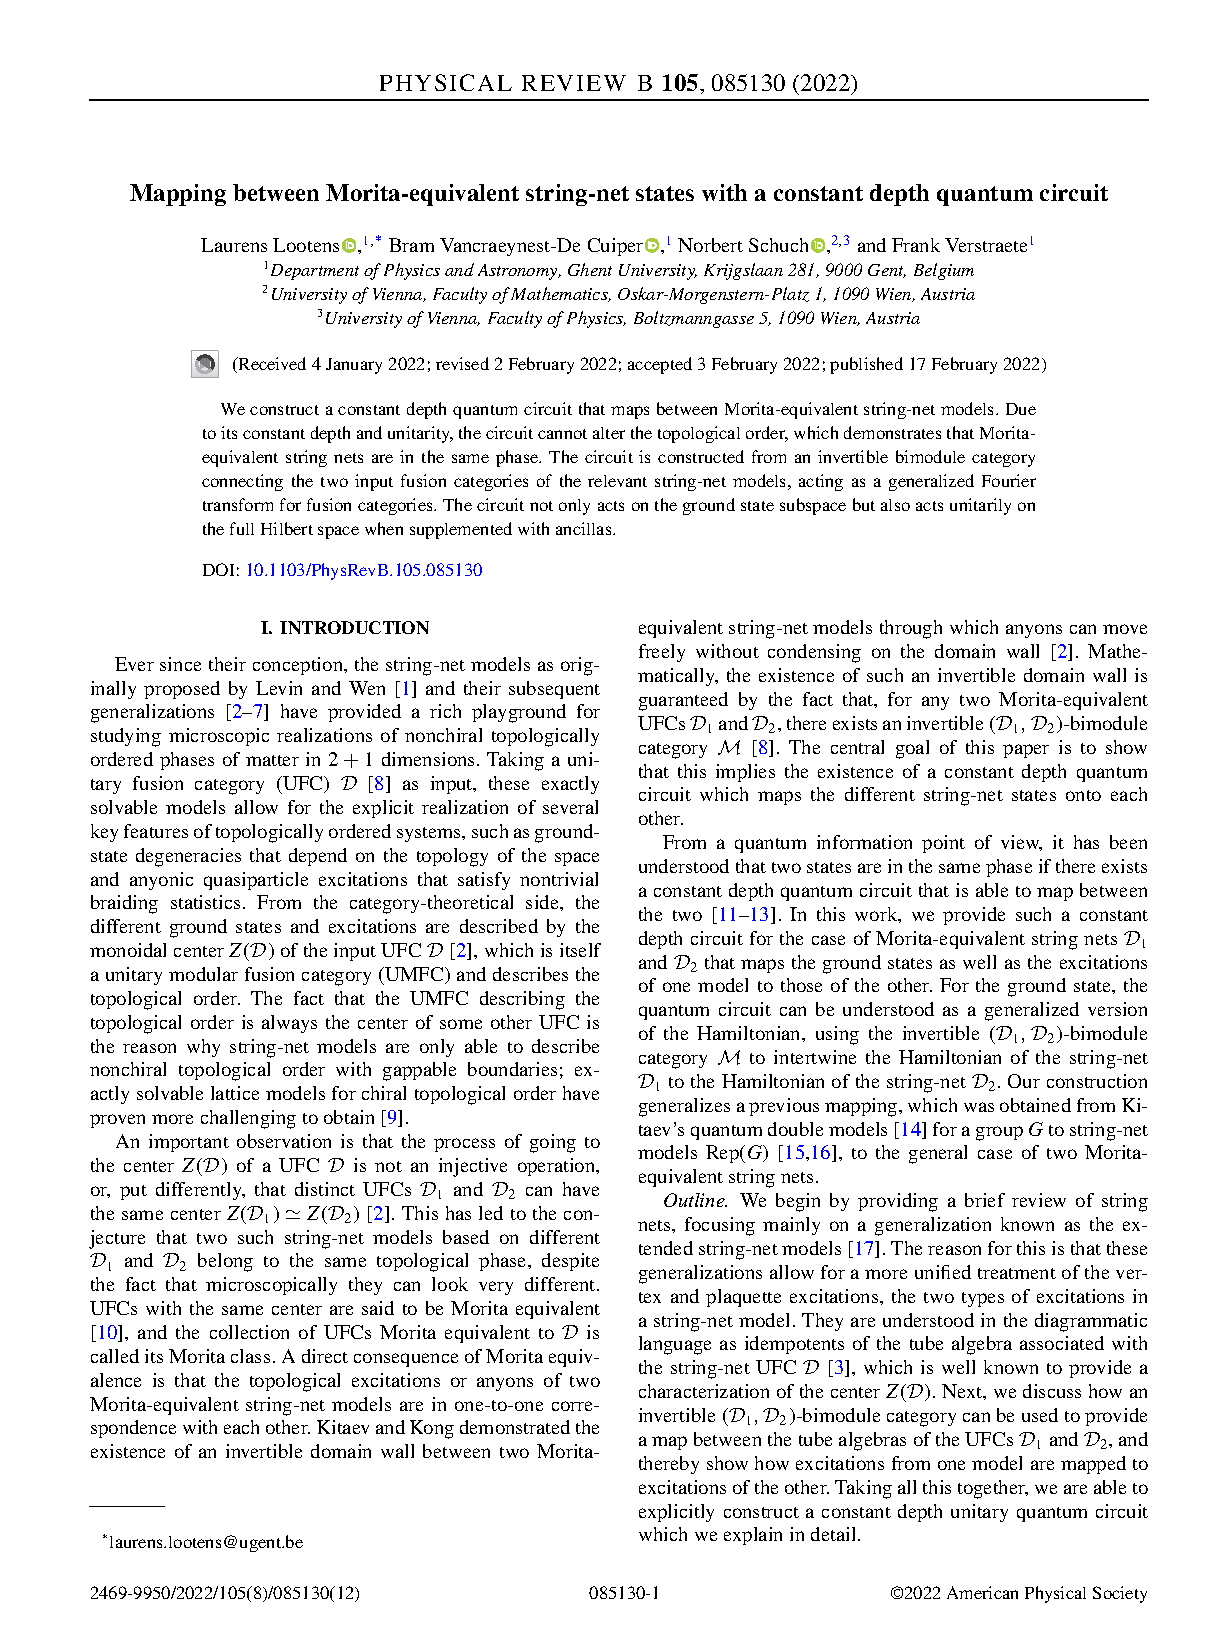
\includepdf[pages=-, trim=0 1.2cm 0 0, clip=true, frame=false, noautoscale=true, width=1.14\headwidth, offset=-4mm 6mm, , pagecommand={}]{papers/string_net}
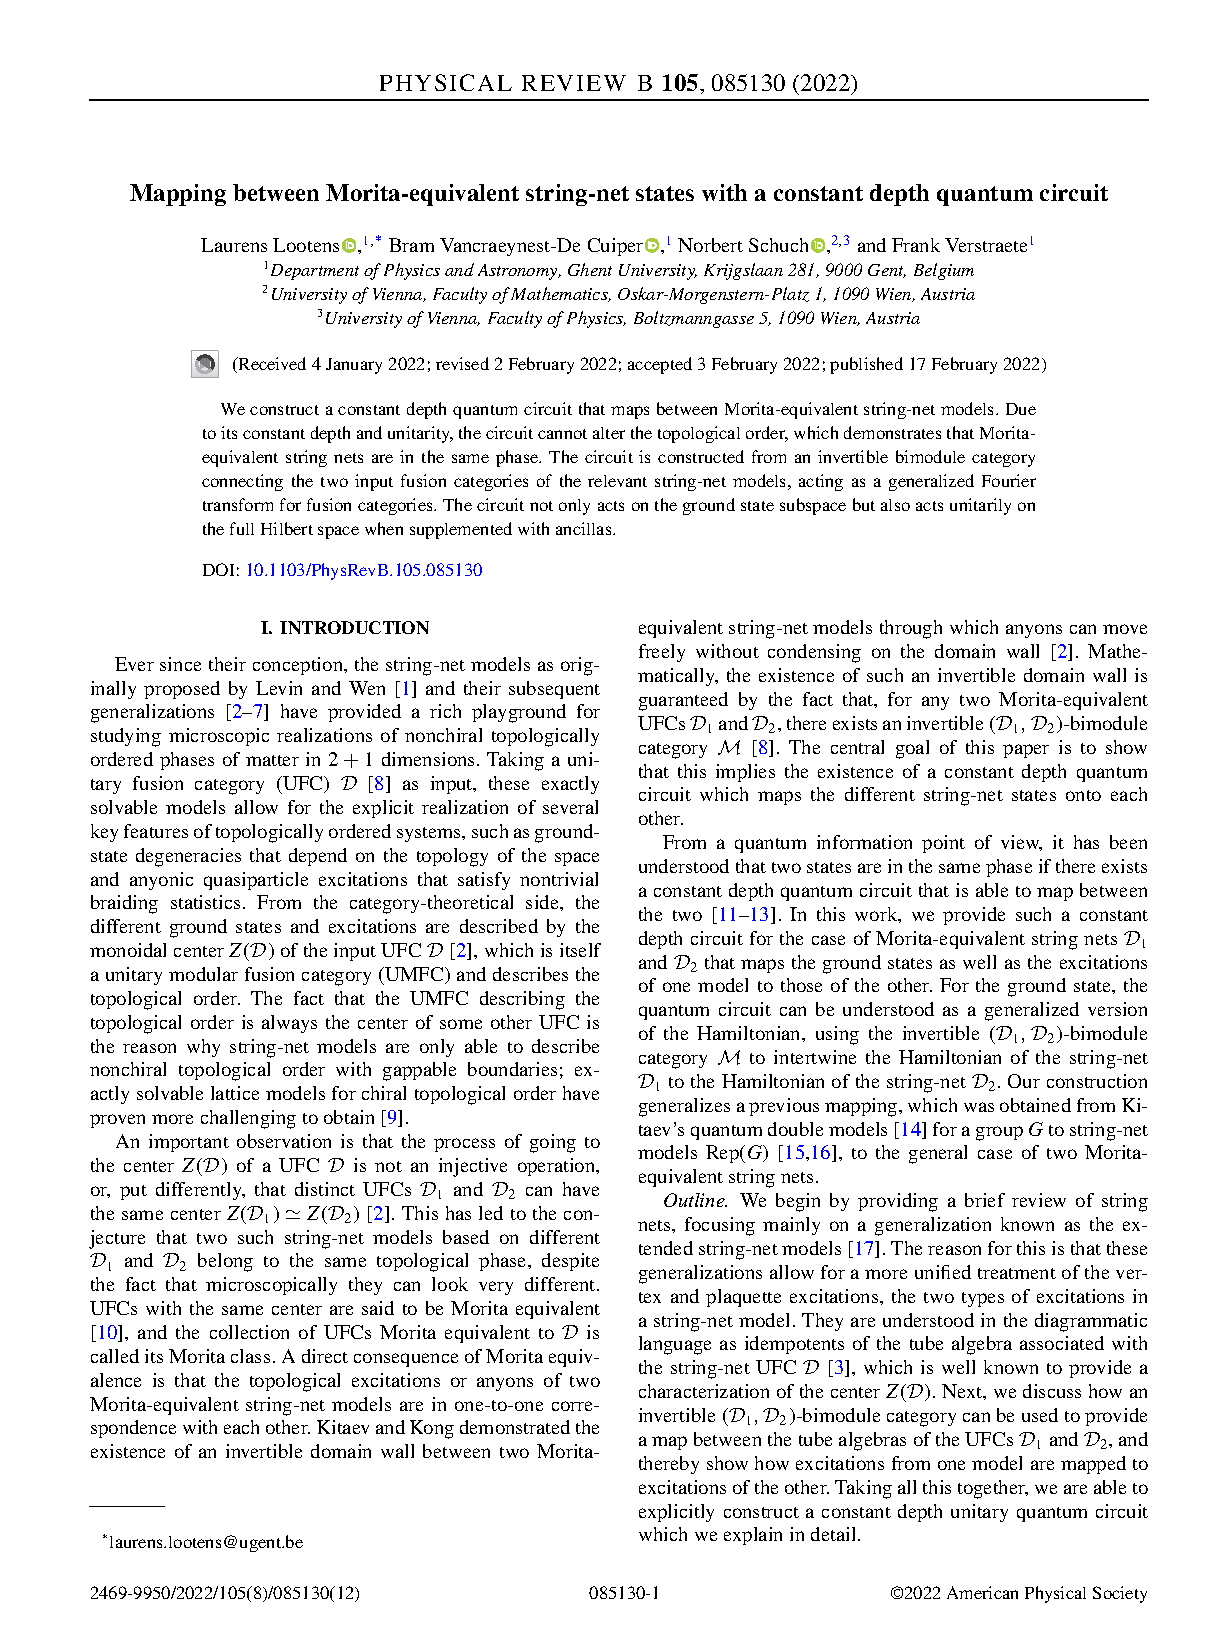
\includepdf[pages=-,
trim=12mm 12.7mm 12mm 9.2mm, clip=true,
noautoscale=true, width=\textwidth,
offset=-0.65mm 5mm,
pagecommand={\thispagestyle{publication}}]{papers/string_net}